% K41_Variational_Minimiser_v1_en.tex
% Paper A: The K41 Spectrum as the Unique Variational Minimiser
%          of a Scale-Resolved Free Energy
% Author: Lukas Geiger, 2026

\documentclass[12pt,a4paper]{article}
\usepackage[utf8]{inputenc}
\usepackage[T1]{fontenc}
\usepackage[english]{babel}
\usepackage{lmodern}
\usepackage{microtype}
\usepackage{amsmath,amssymb,amsthm,mathrsfs}
\usepackage{mathtools}
\usepackage{enumitem}
\usepackage{array}
\usepackage{xcolor}
\usepackage{geometry}
\geometry{a4paper, margin=2.5cm}
\setlength{\emergencystretch}{3em}
\usepackage{tikz}
\usetikzlibrary{arrows.meta,positioning,calc}
\usepackage{xurl}
\usepackage[unicode=true]{hyperref}
\hypersetup{
  colorlinks=true,
  linkcolor=blue!70!black,
  citecolor=green!50!black,
  urlcolor=blue!70!black,
  pdftitle={The K41 Spectrum as the Unique Variational Minimiser of a Scale-Resolved Free Energy},
  pdfauthor={Lukas Geiger},
  pdfsubject={Variational characterisation of the Kolmogorov K41 energy spectrum},
  pdfkeywords={K41 spectrum, turbulence, variational principle, free energy, Kolmogorov scaling}
}
\providecommand*{\HyperDestNameFilter}[1]{en.#1}
\Urlmuskip=0mu plus 2mu\relax
\newcolumntype{L}[1]{>{\raggedright\arraybackslash}p{#1}}

\theoremstyle{definition}
\newtheorem{definition}{Definition}[section]
\theoremstyle{plain}
\newtheorem{theorem}[definition]{Theorem}
\newtheorem{lemma}[definition]{Lemma}
\newtheorem{proposition}[definition]{Proposition}
\newtheorem{corollary}[definition]{Corollary}
\newtheorem{conjecture}[definition]{Conjecture}
\newtheorem{axiom}[definition]{Axiom}
\theoremstyle{remark}
\newtheorem{remark}[definition]{Remark}

% ---------------------------------------------------------------------------
\title{The K41 Spectrum as the Unique Variational Minimiser\\
of a Scale-Resolved Free Energy}

\author{Lukas Geiger\\
\textit{Independent Researcher, Bernau, Germany}\\
ORCID: \href{https://orcid.org/0009-0005-7296-1534}{0009-0005-7296-1534}}

\date{May 2026}

\begin{document}
\maketitle

% ===================================================================
\begin{abstract}
We formulate and prove a reference-normalised variational principle that characterises
the Kolmogorov $k^{-5/3}$ energy spectrum as the unique energy-profile
minimiser of a scale-resolved free-energy functional within the stated
K41-normalised admissible class.  Starting from a
Littlewood--Paley decomposition of the velocity field, we define a
free-energy functional $\mathcal{F}[\mathbf{E}]$ based on the
Kullback--Leibler divergence between the shell-energy distribution and a
K41 reference equilibrium.  We introduce the K41-normalised class of
admissible energy-flux operators---local, dimensionally consistent,
monotone closures satisfying axioms (A1) and (A3) together with the
normalisation condition in Definition~\ref{def:admissible}---and prove
that the K41 distribution is the unique minimiser of
$\mathcal{F}[\mathbf{E}]$ over the joint feasible set of energy profiles
and closures, subject to constant scale-to-scale energy flux
(Theorem~\ref{thm:K41}).  The
minimiser is non-degenerate: the Hessian of $\mathcal{F}$ at
$\mathbf{E}^*$ is diagonal with entries $1/E_j^* > 0$, providing
  shell-energy stiffness that grows as $k_j^{2/3}$ for dyadic shells.  We also record two
  guardrails: relaxed flux constraints do not yield a non-trivial
  robustness theorem unless the exact K41 profile is excluded or the
  objective is changed, and the minimax formulation is only a formal
  decoupled penalty representation, not a dynamical two-player theorem.
Under additional Gaussian/log-normal fluctuation assumptions, Hessian
fluctuations around the variational minimum lead to the
Kolmogorov--Obukhov (K62) exponent formula.  The result is unconditional
only as a static finite/inertial-range variational statement inside the
stated K41-normalised class; it is not a dynamical Navier--Stokes
selection theorem.  Anomalous dissipation under additional hypotheses on
the nonlinear cascade is treated separately in a companion
paper~\cite{Geiger2026b}.
\end{abstract}

\begin{center}
\small\emph{Preprint note. This is Paper A in the turbulence split. It isolates the static, reference-normalised K41 variational-minimiser theorem. The companion Paper B treats anomalous dissipation and the Downhill Flux Condition as a conditional cascade route.}
\end{center}
\clearpage

% ===================================================================
\section{Introduction}\label{sec:intro}

Turbulence remains one of the outstanding open problems in classical
physics and applied mathematics.  Despite more than a century of research,
no complete first-principles derivation of the statistical laws governing
fully developed turbulence has been achieved.

\subsection{The Kolmogorov theory}

In his landmark 1941 papers, Kolmogorov~\cite{K41a,K41b} postulated that
in the inertial range of fully developed, homogeneous, isotropic
turbulence, the energy spectrum takes the universal form
\begin{equation}\label{eq:K41}
  E(k) \;=\; C_K \,\varepsilon^{2/3}\, k^{-5/3},
\end{equation}
where $\varepsilon$ denotes the mean rate of energy dissipation per unit
mass and $C_K \approx 1.5$ is the Kolmogorov constant.  This prediction,
derived from dimensional analysis and the hypothesis of local isotropy,
is well supported experimentally and numerically across a broad range of
Reynolds numbers~\cite{Frisch95,Pope00}.

\subsection{Our contribution}

In this paper we take a different approach.  Rather than deriving the
K41 spectrum from dimensional analysis alone, we show that it is the
\emph{free-energy preferred} distribution inside the stated K41-normalised
constant-flux comparison class.
We introduce a free-energy functional~$\mathcal{F}$ on the space of
scale-resolved energy distributions and prove:
\begin{enumerate}
  \item The K41 spectrum is the \emph{unique} minimiser of $\mathcal{F}$
        under the constraint of constant energy flux, where the minimisation
        runs jointly over K41-normalised admissible local flux operators and
        energy profiles (Theorem~\ref{thm:K41}).  The argument does not
        presuppose a single fixed closure, but it remains explicitly
        reference-normalised.
  \item The minimiser is non-degenerate, with the Hessian providing
        scale-dependent shell-energy stiffness $1/E_j^* \propto k_j^{2/3}$ that
        penalises small-scale perturbations more severely than large-scale
        ones---a static convex signature compatible with downscale cascade
        bias.
  \item Relaxed flux constraints and the minimax notation are recorded as
        scope guardrails: if the exact K41 profile remains feasible, the
        relaxed problem is trivial, and the minimax form is a decoupled
        penalty representation rather than a dynamical two-player theorem
        (Propositions~\ref{prop:dfc-slack}--\ref{prop:minimax}).
\end{enumerate}
The dynamical consequences of the free-energy structure, including
anomalous dissipation under additional hypotheses on the nonlinear
cascade, will be developed in a companion paper~\cite{Geiger2026b}.

\subsection{Structural classification}

Within the broader programme of free-energy spectral
theory~\cite{FST-Unified2026}, the K41 selection mechanism exhibits the
\textbf{Pattern~A stability logic}: (a)~the leading-order energy budget is
neutral (any power-law spectrum is kinematically admissible); (b)~the
first-order constant-flux constraint restricts but does not uniquely
determine the profile; (c)~the second-order strict convexity
of~$\mathcal{F}$ selects K41 as the unique minimiser.  This three-level
hierarchy is discussed in Section~\ref{sec:resolvent-cascade}.

This paper is self-contained; all main results depend only on definitions
and proofs within this document. Connections to the broader FST programme
are cited for context but are not logically required.

For orientation, Table~\ref{tab:claim-status-ledger} separates the
paper's theorem-level content from its diagnostic and open bridge
components.  This is the intended reading order: the variational theorem is
closed inside the stated class, while the numerical, intermittency and DNS
items remain support layers or future gates.

\begin{table}[ht]
\centering
\small
\setlength{\tabcolsep}{4pt}
\begin{tabular}{|L{0.21\textwidth}|L{0.35\textwidth}|L{0.33\textwidth}|}
\hline
\textbf{Component} & \textbf{Evidence or presentation layer} & \textbf{Current status and caveat} \\
\hline
Static variational core & KL functional, admissible flux family and joint feasible-set proof. & Proved within the K41-normalised inertial shell class; not an intrinsic DNS or Navier--Stokes selection theorem. \\
\hline
Local stiffness & Diagonal Hessian at $\mathbf{E}^*$ with shell-energy scale $1/E_j^* \propto k_j^{2/3}$. & Proved as local convexity; it supplies static stiffness, not return dynamics. \\
\hline
Guardrail branches & Relaxed-flux and minimax propositions. & Scope controls only; they do not add a positive robustness theorem or a dynamical game. \\
\hline
Synthetic numerics & Six model spectra and $300$ random perturbation tests from \texttt{compute\_F\_spectrum.py}. & Illustration and audit check; not independent empirical validation. \\
\hline
K62 / intermittency link & Gaussian/log-normal fluctuation route around the Hessian scale. & Formal model route; a cascade measure and structure-function bridge are still required. \\
\hline
DNS and Paper-B bridge & Proposed DNS protocol and companion cascade paper. & Future or conditional layer; depends on DFC and nonlinear-cascade hypotheses outside this paper. \\
\hline
\end{tabular}
\caption{Claim-status ledger for the K41 variational-minimiser paper.}
\label{tab:claim-status-ledger}
\end{table}

% ===================================================================
% Figure 1: Proof chain overview
% ===================================================================
\begin{figure}[ht]
\centering
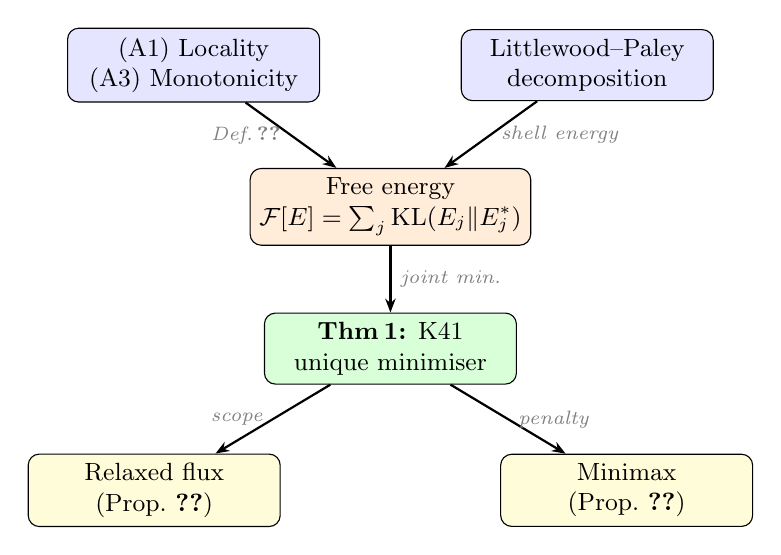
\begin{tikzpicture}[
  box/.style={draw, rounded corners, minimum width=3.2cm, minimum height=0.9cm,
              align=center, font=\small},
  arrow/.style={-{Stealth[length=5pt]}, thick},
  note/.style={font=\scriptsize\itshape, text=gray}
]
% Row 1: Axioms
\node[box, fill=blue!10] (A1) at (0,0) {(A1) Locality\\(A3) Monotonicity};
\node[box, fill=blue!10] (LP) at (5,0) {Littlewood--Paley\\decomposition};

% Row 2: Functional
\node[box, fill=orange!15] (F) at (2.5,-1.8) {Free energy\\$\mathcal{F}[E] = \sum_j \mathrm{KL}(E_j \| E_j^*)$};

% Row 3: Main Theorem
\node[box, fill=green!15] (T1) at (2.5,-3.6) {\textbf{Thm\,1:} K41\\unique minimiser};

% Row 4: Extensions
\node[box, fill=yellow!15] (R) at (-0.5,-5.4) {Relaxed flux\\(Prop.~\ref{prop:dfc-slack})};
\node[box, fill=yellow!15] (M) at (5.5,-5.4) {Minimax\\(Prop.~\ref{prop:minimax})};

% Arrows
\draw[arrow] (A1) -- (F) node[midway, left, note] {Def.\,\ref{def:F}};
\draw[arrow] (LP) -- (F) node[midway, right, note] {shell energy};
\draw[arrow] (F) -- (T1) node[midway, right, note] {joint min.};
\draw[arrow] (T1) -- (R) node[midway, left, note] {scope};
\draw[arrow] (T1) -- (M) node[midway, right, note] {penalty};
\end{tikzpicture}
\caption{Logical structure of the proof.  The free energy functional
$\mathcal{F}[\mathbf{E}]$ is constructed from the Littlewood--Paley
decomposition and the admissible flux family (axioms A1, A3).
Theorem~\ref{thm:K41} (K41 uniqueness) follows from joint minimisation.
The relaxed-flux and minimax branches record scope guardrails and a formal
penalty representation, not additional dynamical theorems.}
\label{fig:proof-chain}
\end{figure}

% ===================================================================
\section{The Scale-Resolved Free-Energy Functional}\label{sec:functional}

\subsection{Littlewood--Paley decomposition}

Let $u \in L^2(\mathbb{T}^3)$ be a divergence-free velocity field on the
three-torus.  We employ the standard Littlewood--Paley decomposition
\begin{equation}\label{eq:LP}
  u \;=\; \sum_{j \ge -1} \Delta_j u,
\end{equation}
where $\Delta_j$ is the frequency-localisation operator at dyadic shell
$|\xi| \sim 2^j$.  We set $k_j = 2^j$ and define the \emph{shell energy}
\begin{equation}\label{eq:Ej}
  E_j \;:=\; \|\Delta_j u\|_{L^2}^2.
\end{equation}
In the inertial range, the K41 prediction~\eqref{eq:K41} translates to
\begin{equation}\label{eq:Ej_star}
  E_j^* \;=\; C_K\, \varepsilon^{2/3}\, k_j^{-5/3} \,\Delta k_j,
  \qquad \Delta k_j = k_j \ln 2 \quad (\text{dyadic shell width}).
\end{equation}

\subsection{Energy flux constraint}

The scale-to-scale energy flux through wavenumber $k_j$ is defined via the
trilinear term in the Navier--Stokes equations:
\begin{equation}\label{eq:flux}
  \Pi_j \;=\; -\sum_{\ell \le j}
    \langle \Delta_\ell(u \cdot \nabla u),\; \Delta_\ell u \rangle.
\end{equation}
In the inertial range, a statistically stationary cascade satisfies
\begin{equation}\label{eq:const_flux}
  \Pi_j \;=\; \varepsilon \quad \text{for all } j_{\mathrm{in}} \le j \le j_{\mathrm{dis}}.
\end{equation}

\subsection{The functional}

\begin{definition}[Scale-resolved free energy]\label{def:F}
Let $\mathbf{E} = (E_j)_{j \in \mathcal{J}}$ be a distribution of shell
energies over the inertial range $\mathcal{J} = \{j_{\mathrm{in}}, \dots,
j_{\mathrm{dis}}\}$, with $E_j > 0$.  Let $\mathbf{E}^* = (E_j^*)$ be
the Kolmogorov reference distribution~\eqref{eq:Ej_star}.  The
\emph{scale-resolved free-energy functional} is
\begin{equation}\label{eq:F}
  \mathcal{F}[\mathbf{E}]
  \;:=\;
  \sum_{j \in \mathcal{J}}
  \Bigl[
    E_j \ln\!\frac{E_j}{E_j^*} \;-\; E_j \;+\; E_j^*
  \Bigr].
\end{equation}
\end{definition}

\begin{remark}
The summand $f(E_j) = E_j \ln(E_j/E_j^*) - E_j + E_j^*$ is the
Kullback--Leibler divergence (relative entropy) of the pair $(E_j, E_j^*)$
when viewed as unnormalised measures on a single-point space.  It satisfies
$f(E_j) \ge 0$ with equality if and only if $E_j = E_j^*$.  Hence
$\mathcal{F}[\mathbf{E}] \ge 0$ with equality if and only if $\mathbf{E}
= \mathbf{E}^*$.
\end{remark}

\begin{figure}[ht]
\centering
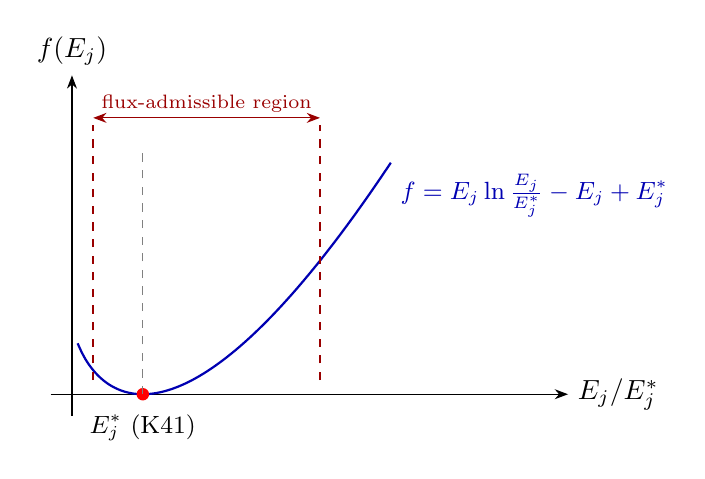
\begin{tikzpicture}[scale=0.9]
% Axes
\draw[-{Stealth}] (-0.3,0) -- (7,0) node[right] {$E_j / E_j^*$};
\draw[-{Stealth}] (0,-0.3) -- (0,4.5) node[above] {$f(E_j)$};
% KL curve: f(x) = x ln(x) - x + 1, plotted for x = E_j/E_j*
\draw[thick, blue!70!black, domain=0.08:4.5, smooth, samples=80]
  plot ({\x}, {\x*ln(\x)/ln(2.718) - \x + 1});
% Minimum point
\fill[red] (1,0) circle (2.5pt);
\node[below, font=\small] at (1,-0.15) {$E_j^*$ (K41)};
% Annotation
\draw[dashed, gray] (1,0) -- (1,3.5);
\node[font=\small, text=blue!70!black, right] at (4.5,2.8) {$f = E_j\ln\frac{E_j}{E_j^*} - E_j + E_j^*$};
% Flux constraint region
\draw[thick, red!60!black, dashed] (0.3,0.2) -- (0.3,3.8);
\draw[thick, red!60!black, dashed] (3.5,0.2) -- (3.5,3.8);
\node[font=\scriptsize, text=red!60!black] at (1.9,4.1) {flux-admissible region};
\draw[{Stealth}-{Stealth}, red!60!black] (0.3,3.9) -- (3.5,3.9);
\end{tikzpicture}
\caption{The free-energy density $f(E_j) = E_j \ln(E_j / E_j^*) - E_j + E_j^*$
as a function of the shell energy ratio $E_j / E_j^*$. The unique global minimum
at $E_j = E_j^*$ (K41 spectrum) is marked. The flux constraint restricts the
admissible region, but the minimum lies inside for the K41-normalised
comparison class, illustrating K41 as the joint energy minimiser.}
\label{fig:FE-landscape}
\end{figure}

\subsection{Dimensional consistency}

We verify that $\mathcal{F}$ is dimensionally consistent.  Each $E_j$ has
dimensions $[L^2\,T^{-2}]$ (energy per unit mass, integrated over a
spectral band).  Since $E_j^*$ shares the same dimensions, the ratio
$E_j/E_j^*$ is dimensionless, the logarithm is well-defined, and each
summand in~\eqref{eq:F} has dimensions $[L^2\,T^{-2}]$.

% ===================================================================
\section{Main Results}\label{sec:results}

\subsection{Uniqueness of Kolmogorov scaling}

\begin{definition}[Admissible flux family]\label{def:admissible}
A family of flux operators $\bigl(\Pi_j[\mathbf{E}]\bigr)_{j \in
\mathcal{J}}$ is called \emph{admissible} if each $\Pi_j$ satisfies:
\begin{enumerate}
  \item[\textup{(A1)}] \textbf{Locality.}\;
    $\Pi_j$ depends only on $E_{j-1},\, E_j,\, E_{j+1}$.
  \item[\textup{(A2)}] \textbf{Dimensional consistency.}\;
    $[\Pi_j] = [E_j / \tau_j]$ with the eddy turnover time
    $\tau_j = (k_j^2\,E_j)^{-1/2}$, so that $\Pi_j$ has the form
    \begin{equation}\label{eq:closure_general}
      \Pi_j[\mathbf{E}]
      \;=\;
      k_j\,E_j^{3/2}\;\Phi_j\!\Bigl(
        \frac{E_{j-1}}{E_j},\;
        \frac{E_{j+1}}{E_j}
      \Bigr),
    \end{equation}
    where $\Phi_j : (0,\infty)^2 \to (0,\infty)$ is a smooth
    dimensionless function satisfying $\Phi_j(r^*_{-},\, r^*_{+}) = \alpha$
    for some universal constant $\alpha > 0$, with
    $r^*_{\pm} = E_{j \pm 1}^* / E_j^*$.
  \item[\textup{(A3)}] \textbf{Monotonicity.}\;
    $\partial \Pi_j / \partial E_j > 0$ for all $\mathbf{E} > 0$.
\end{enumerate}
We denote the set of all admissible families by $\mathscr{A}$.
\end{definition}

\begin{remark}[Reference-normalised admissible class]\label{rem:reference-normalised-class}
The condition $\Phi_j(r^*_{-},r^*_{+})=\alpha$ normalises the admissible
class at the K41 reference profile.  The theorem below is therefore a
relative selection theorem inside this stated K41-normalised class.  It
does not assert that every fixed local monotone closure selects K41, nor
does it exclude alternative closure families normalised around a different
reference profile.  Such alternatives would require additional
scale-invariance, universality, or empirical admissibility assumptions.
\end{remark}

\begin{proposition}[Dimensional derivation of the flux prefactor]\label{prop:A2-derived}
Within the reduced scale-local inertial shell ansatz in which the only
dimensional variables admitted at shell~$j$ are $k_j$ and $E_j$, the
prefactor in Axiom~\textup{(A2)} follows from dimensional analysis:
$\Pi_j = k_j\,E_j^{3/2}\,\Phi_j(\cdot)$.  Thus (A2) is the canonical
prefactor inside this stipulated ansatz, not a theorem excluding richer
closure classes with additional dimensional or dimensionless parameters.
\end{proposition}

\begin{proof}
Inside this reduced ansatz, Buckingham's $\Pi$-theorem forces the flux
$\Pi_j$ to be a product of powers of the admitted dimensional quantities
$k_j$ and~$E_j$, multiplied by a dimensionless function of dimensionless
ratios. Write $\Pi_j = k_j^{a}\,E_j^{b}\,\Phi_j(\ldots)$ with
$[\Pi_j] = [L^2\,T^{-3}]$ (energy flux per unit mass),
$[k_j] = [L^{-1}]$, and $[E_j] = [L^2\,T^{-2}]$.

Dimensional matching: $[k_j^a\,E_j^b] = L^{-a}\,L^{2b}\,T^{-2b} = L^{2b-a}\,T^{-2b}$.

Setting equal to $L^2\,T^{-3}$:
\[
2b - a = 2, \qquad 2b = 3 \quad\Longrightarrow\quad b = \tfrac{3}{2},\;\; a = 1.
\]
Hence $\Pi_j = k_j\,E_j^{3/2}\,\Phi_j$, and by~(A1) the dimensionless
function $\Phi_j$ can depend only on the local ratios $E_{j-1}/E_j$ and
$E_{j+1}/E_j$. The eddy turnover time
$\tau_j = (k_j^2\,E_j)^{-1/2}$ is likewise the canonical local timescale
inside the same restricted set of dimensional variables.  Closures that
retain viscosity, forcing scales, intermittency variables, or further
dimensionless shell parameters lie outside this particular reduction.
\end{proof}

\begin{remark}
The classical Kolmogorov--Heisenberg closure $\Pi_j = \alpha\,k_j\,E_j^{3/2}$
corresponds to the special case $\Phi_j \equiv \alpha$~\cite{MY75}.  Definition~\ref{def:admissible}
enlarges the model class beyond this single algebraic relation and is
designed to cover local closure motifs such as EDQNM-type closures,
Leith-type diffusion models, and truncated triad interactions when they
are expressed in the shell variables of Definition~\ref{def:admissible}.
The family $\mathscr{A}$ is therefore a structured local comparison class
rather than a single closure model.
Proposition~\ref{prop:A2-derived} separates the reduced inertial
dimensional ansatz from the genuinely variable assumptions of locality
and monotonicity.  It therefore clarifies the modelling content of (A2)
rather than removing all independent modelling content from the flux
prefactor.
\end{remark}

\begin{theorem}[Relative uniqueness in the K41-normalised admissible class]\label{thm:K41}
Let $\varepsilon > 0$ be given and let $\mathscr{A}$ be the class of
admissible flux families (Definition~\ref{def:admissible}), including its
K41 normalisation condition.
Consider the \emph{joint} minimisation problem
\begin{equation}\label{eq:min}
  \min_{\substack{\mathbf{E} > 0,\\ \Pi \in \mathscr{A}}}
  \;\mathcal{F}[\mathbf{E}]
  \qquad \text{subject to} \quad
  \Pi_j[\mathbf{E}] = \varepsilon
  \;\;\text{for all } j \in \mathcal{J}.
\end{equation}
Then:
\begin{enumerate}
  \item[\textup{(i)}]
    In the joint feasible set
    $\{(\mathbf{E},\Pi):\Pi\in\mathscr{A},\;
    \Pi_j[\mathbf{E}]=\varepsilon\;\text{for all }j\}$, the K41
    distribution
    $E_j^* = C_K\,\varepsilon^{2/3}\,k_j^{-5/3}\,\Delta k_j$
    is the unique minimiser of~$\mathcal{F}$ in the energy variable, and
    the minimum is realised
    by the Kolmogorov--Heisenberg member $\Phi_j \equiv \alpha$ with
    $C_K = \bigl(\alpha\,(\ln 2)^{3/2}\bigr)^{-2/3}$.
  \item[\textup{(ii)}]
    The energy minimiser is non-degenerate: the Hessian
    $D^2\mathcal{F}|_{\mathbf{E}^*}$ restricted to the tangent space of
    the joint feasible set in the energy directions is strictly positive
    definite. (This is a direct consequence of the strict convexity of
    the KL divergence; its content is the scale-dependent stiffness
    $1/E_j^* \propto k_j^{2/3}$ for dyadic shell energies, see Step~5b below.)
\end{enumerate}
\end{theorem}

\begin{proof}
\textbf{Step 1: Joint feasible profiles.}\;
We restrict attention to pairs $(\mathbf{E},\Pi)$ in the joint feasible set
for which $\Pi\in\mathscr{A}$ and $\Pi_j[\mathbf{E}]=\varepsilon$ for all
$j$.  Local monotonicity in $E_j$ is not, by itself, a global existence
theorem for the coupled shell system; existence for a specific fixed
closure is therefore treated only as a feasibility issue.  The theorem
does not claim that every fixed closure selects K41.

\textbf{Step 2: Lower bound via convexity.}\;
Since, in the standard terminology of convex analysis and perturbation theory~\cite{Rockafellar70,BonnansShapiro00}, each summand $f(E_j) = E_j\ln(E_j/E_j^*) - E_j + E_j^*$ is
strictly convex with global minimum $f(E_j^*) = 0$, we have
\begin{equation}\label{eq:F_lower}
  \mathcal{F}[\mathbf{E}]
  \;\ge\; 0
  \;=\; \mathcal{F}[\mathbf{E}^*],
\end{equation}
with equality if and only if $E_j = E_j^*$ for all~$j$.

\textbf{Step 3: Attainability.}\;
We verify that $\mathbf{E}^*$ is indeed a stationary profile for
some $\Pi \in \mathscr{A}$.  Choose the Kolmogorov--Heisenberg closure
$\Phi_j \equiv \alpha$.  Then
\[
  \Pi_j[\mathbf{E}^*]
  \;=\; \alpha\,k_j\,(E_j^*)^{3/2}
  \;=\; \alpha\,k_j\,
    \bigl(C_K\,\varepsilon^{2/3}\,k_j^{-5/3}\,k_j\ln 2\bigr)^{3/2}
  \;=\; \alpha\,C_K^{3/2}\,(\ln 2)^{3/2}\,\varepsilon.
\]
Setting $C_K = \bigl(\alpha\,(\ln 2)^{3/2}\bigr)^{-2/3}$ yields
$\Pi_j[\mathbf{E}^*] = \varepsilon$.  (The geometric factor $(\ln 2)^{3/2}$
arising from the dyadic shell width is absorbed into the Kolmogorov
constant $C_K$, which is thereby determined by the closure
parameter~$\alpha$.)  Hence the lower bound~\eqref{eq:F_lower} is
attained.

\textbf{Step 4: Uniqueness.}\;
Suppose $\Pi' \in \mathscr{A}$ and $\mathbf{E}' \ne \mathbf{E}^*$ form a
joint feasible pair, i.e.\ $\Pi'_j[\mathbf{E}'] = \varepsilon$.  Then strict convexity gives
$\mathcal{F}[\mathbf{E}'] > 0 = \mathcal{F}[\mathbf{E}^*]$, so $\mathbf{E}'$
cannot be a minimiser of~\eqref{eq:min}.  Hence $\mathbf{E}^*$ is the
\emph{unique energy profile} solving the joint problem.

\smallskip\noindent
\textbf{Note on the logical structure.}\;
The uniqueness in Step~4 follows from the strict positivity of the KL
divergence away from the reference, which holds for \emph{any} choice
of~$\mathbf{E}^*$. The physically non-trivial content resides in
Step~3 (attainability): within the K41-normalised class, there exists an
admissible closure realising $\Pi_j[\mathbf{E}^*] = \varepsilon$.
References such as $k^{-3}$ are not excluded by KL convexity alone; they
would require a different normalisation or stronger scale-invariance and
uniformity assumptions on the closure family (see
Remarks~\ref{rem:reference-normalised-class} and~\ref{rem:circularity}).

\textbf{Step 5: Non-degeneracy.}\;
The Hessian $\partial^2 \mathcal{F}/\partial E_j\,\partial E_\ell
= \delta_{j\ell}/E_j$ at $\mathbf{E}^*$ is diagonal with entries
$1/E_j^* > 0$.  For a \emph{fixed} closure $\Pi \in \mathscr{A}$, the
constraint $\Pi_j[\mathbf{E}] = \varepsilon$ imposes $|\mathcal{J}|$
equations on $|\mathcal{J}|$ unknowns, generically yielding isolated
solutions, so that the tangent space of the constraint manifold at
$\mathbf{E}^{(\Pi)}$ is trivial and non-degeneracy is vacuously satisfied.
The substantive content of~(ii) concerns the \emph{joint} problem: in the
extended space $(\mathbf{E}, \Pi)$ with $\Pi$ varying over the
(infinite-dimensional) family~$\mathscr{A}$, the constraint set
$\{(\mathbf{E}, \Pi) : \Pi_j[\mathbf{E}] = \varepsilon\}$ has tangent
directions along which $\Pi$ varies.  The unrestricted Hessian
$D^2_{\mathbf{E}}\mathcal{F}|_{\mathbf{E}^*}$ is strictly positive
definite (diagonal entries $1/E_j^* > 0$), hence its restriction to
\emph{any} subspace remains positive definite.

\medskip
\noindent\textbf{Step 5b: Second-order interpretation.}\;
Since $E_j^* = C_K\varepsilon^{2/3}k_j^{-5/3}\Delta k_j
      = C_K\varepsilon^{2/3}(\ln 2)k_j^{-2/3}$ on dyadic shells,
the diagonal entries $1/E_j^* \propto k_j^{2/3}$ of the Hessian grow with
wavenumber.  Thus small-scale perturbations of the K41 shell-energy profile
are penalised more severely than large-scale ones.  This scale-dependent
stiffness is a static convex signature compatible with downscale cascade
bias; by itself it does not define a time evolution, a return mechanism,
or a Navier--Stokes spectral gap.  The one-parameter
freedom in the Kolmogorov--Heisenberg closure ($\Phi_j \equiv \alpha$)
corresponds to a single flat direction in the $\Pi$-fibre of the
extended space $(\mathbf{E}, \Pi)$, which does not affect the strict
positivity of $D^2_{\mathbf{E}}\mathcal{F}$.  This structure is an
instance of the second-order resolvent dominance pattern discussed
in~\cite{FST-Unified2026}.
\end{proof}

\begin{remark}[Diagonal Hessian bound]\label{rem:hessian}
The Hessian of $\mathcal{F}$ at the K41 minimiser is diagonal with entries
\[
  \frac{\partial^2\mathcal{F}}{\partial E_j^2}
  \;=\; \frac{1}{E_j^*}.
\]
Consequently,
\[
  \min_j\frac{1}{E_j^*}
  \;=\;
  \frac{1}{C_K\,\varepsilon^{2/3}\,k_1^{-5/3}\,\Delta k_1}
  \;=\;
  \frac{1}{C_K\,\varepsilon^{2/3}(\ln 2)\,k_1^{-2/3}}
  \;>\; 0.
\]
This provides the local weighted stability scale of the variational
functional.  It should not be read, by itself, as a spectral gap theorem
for the Navier--Stokes dynamics.
\end{remark}

\begin{remark}[On the role of the reference spectrum]\label{rem:circularity}
A natural objection is that the KL functional $\mathcal{F}$ is
\emph{minimised at} $\mathbf{E}^*$ \emph{by construction}, regardless
of the physical content of~$\mathbf{E}^*$.  Indeed, for any fixed
closure $\Pi$, the unconstrained minimum of $\mathcal{F}$ is always
$\mathbf{E}^*$.  The non-trivial content of Theorem~\ref{thm:K41} is
therefore not that $\mathcal{F}$ achieves its minimum at $\mathbf{E}^*$
--- that is a consequence of the KL construction --- but rather that:
\begin{enumerate}
\item Among all stationary profiles $\mathbf{E}^{(\Pi)}$ (one per closure
  $\Pi \in \mathscr{A}$), only the K41 profile $\mathbf{E}^*$
  \emph{simultaneously satisfies} the constant-flux constraint and
  achieves $\mathcal{F} = 0$.  Every other closure-compatible profile
  has $\mathcal{F} > 0$.
\item The reference $\mathbf{E}^*$ is not arbitrary within the normalised
  Kolmogorov--Heisenberg closure: the constant-flux relation
  $\Pi_j=\alpha k_j E_j^{3/2}=\varepsilon$ fixes the shell energy scaling
  $E_j\propto k_j^{-2/3}$, equivalently the spectral density
  $E(k)\propto k^{-5/3}$.  Broader or differently normalised closure
  families can be designed around other references; the theorem is
  therefore a selection statement inside the stated K41-normalised
  admissible class, not a proof that no other modelling convention can be
  written down.
\end{enumerate}
In summary, the physical input is the constant-flux constraint; the KL
functional provides the selection mechanism among its solution set.
\end{remark}

\begin{remark}[Self-consistency of the K41 reference]
\label{rem:k41-selfconsistency}
The K41 spectrum is used as the reference measure of the KL functional, but
its exponent is also self-consistent with the normalised constant-flux
closure: within the reduced local shell ansatz
$\Pi_j\sim k_j E_j^{3/2}$, constant flux gives
$E_j\propto \varepsilon^{2/3}k_j^{-2/3}$ and hence
$E(k)\propto \varepsilon^{2/3}k^{-5/3}$.  This is a consistency check on
the variational reference, not an independent derivation of all turbulent
statistics.
\end{remark}

\begin{remark}[Heuristic reaction-chain analogy]\label{rem:nash}
The variational structure of Theorem~\ref{thm:K41} admits a useful
heuristic analogy with reaction-chain and game-theoretic language.  Regard
the inertial range as a hierarchical \emph{reaction chain}: large eddies at
scale $k_j$ transfer energy to eddies at scale $k_{j+1}$, each scale acting
as a ``species'' whose fitness is governed by its energy share.  A possible
replicator model on the simplex of normalised shell energies
$p_j = E_j / \sum_\ell E_\ell$ takes the form
\[
  \dot{p}_j
  \;=\;
  p_j\,\bigl(g_j(\mathbf{p}) - \bar{g}(\mathbf{p})\bigr),
\]
where $g_j$ is the net energy gain rate at scale $j$ and $\bar{g}$ the
population average.  With a separately specified payoff compatible with
the KL functional, the K41 profile can be represented as a Nash-type
stationary point and $\mathcal{F}$ can serve as a candidate Lyapunov
function.  This is not part of Theorem~\ref{thm:K41}: no replicator
dynamics, asymptotic stability theorem, or Navier--Stokes return mechanism
is proved here.
\end{remark}

% ===================================================================
\section{Robustness Guardrails and Formal Penalty Structure}\label{sec:robustness}

The strict flux constraint of Theorem~\ref{thm:K41} requires
pointwise $\Pi_j = \varepsilon$ across the inertial range.
In practice, DNS data exhibit small-scale
fluctuations around this idealisation.  We formulate two extensions
  that clarify the scope of finite-Reynolds-number robustness and the
  formal penalty representation of the flux constraint.

\begin{proposition}[Relaxed flux constraint: scope caveat]
\label{prop:dfc-slack}
Let $\mathcal{A}_{\textup{slack}}$ be any relaxed flux-admissible set that
contains the exact K41 profile $\mathbf{E}^*$.  If the objective remains
the same KL functional $\mathcal{F}$, then the minimiser over
$\mathcal{A}_{\textup{slack}}$ is still exactly $\mathbf{E}^*$:
\begin{equation}\label{eq:dfc-slack-bound}
  \arg\min_{\mathbf{E}\in\mathcal{A}_{\textup{slack}}}\mathcal{F}[\mathbf{E}]
  = \mathbf{E}^*.
\end{equation}
Consequently, a non-trivial finite-Reynolds-number slack theorem cannot be
obtained merely by relaxing the flux inequalities while keeping the same
reference-centred objective.  Such a theorem would need an additional
data-fit term, a perturbed reference profile, or empirical bounds that
exclude the exact profile from the feasible comparison class.
\end{proposition}

\begin{proof}
For all positive shell spectra, $\mathcal{F}[\mathbf{E}]\ge0$ and equality
holds only at $\mathbf{E}=\mathbf{E}^*$.  If
$\mathbf{E}^*\in\mathcal{A}_{\textup{slack}}$, then the relaxed infimum is
at most $\mathcal{F}[\mathbf{E}^*]=0$ and at least $0$.  Hence every
relaxed minimiser with objective value zero is $\mathbf{E}^*$.  This proves
the claim and explains why the older ``slack minimiser'' formulation was
too strong: the exact reference profile remains feasible.
\end{proof}

\begin{remark}
Proposition~\ref{prop:dfc-slack} is a guardrail rather than a positive
robustness theorem: finite-Reynolds-number robustness must be formulated
with a perturbed reference, an empirical data-fit term, or a feasible class
that no longer contains the exact K41 profile.  Without such an additional
ingredient, the KL minimum remains exactly at the reference by construction.
\end{remark}

\begin{proposition}[Formal penalty representation]
\label{prop:minimax}
In a finite shell truncation with
$E_{\mathrm{tot}}=\sum_jE_j^*$, the decoupled penalty problem
\begin{equation}\label{eq:minimax}
  \mathbf{E}^*
  \;=\;
  \arg\min_{\mathbf{E} \in \mathcal{E}}\;
  \max_{\boldsymbol{\Pi} \in \mathcal{A}}\;
  \Bigl[
    \mathcal{F}[\mathbf{E}]
    \;-\;
    \lambda \sum_j (\Pi_j - \varepsilon)^2
  \Bigr],
\end{equation}
has the saddle point
$(\mathbf{E}^*,(\varepsilon,\ldots,\varepsilon))$, where
$\mathcal{E}$ is the set of non-negative energy spectra with fixed total
energy and $\mathcal{A}$ is a bounded convex set of admissible flux
profiles.  Since this payoff does not couple $\mathbf{E}$ and
$\boldsymbol{\Pi}$, it is a formal penalty representation of the hard
constraint, not a dynamical two-player theorem for Navier--Stokes transfer.
\end{proposition}

\begin{proof}
We verify the finite-dimensional minimax hypotheses, identify the saddle
point, and make explicit where the representation is decoupled.

\smallskip\noindent
\textbf{Step 1: Strategy spaces.}\;
Define the Lagrangian-penalised payoff
\[
  L(\mathbf{E}, \boldsymbol{\Pi})
  \;:=\;
  \mathcal{F}[\mathbf{E}]
  \;-\;
  \lambda \sum_{j \in \mathcal{J}} (\Pi_j - \varepsilon)^2.
\]
The spectrum variable ranges over
$\mathcal{E} := \{\mathbf{E} \in \mathbb{R}^N_{>0} :
\sum_j E_j = E_{\mathrm{tot}}\}$, the simplex of positive energy
spectra with prescribed total energy $E_{\mathrm{tot}} > 0$ and
  $N = |\mathcal{J}|$ shells.  The flux variable is
  $\boldsymbol{\Pi} = (\Pi_j)_{j=1}^{N-1}$ and ranges over
$\mathcal{A} := \{\boldsymbol{\Pi} \in \mathbb{R}^{N-1} :
0 \le \Pi_j \le \Pi_{\max}\}$ for a fixed upper bound
$\Pi_{\max} > \varepsilon$ (physically, the flux in the inertial range
is bounded above by $O(\varepsilon)$).

The set $\mathcal{E}$ is a compact convex subset of $\mathbb{R}^N$
(it is the intersection of the open positive orthant with the
hyperplane $\sum_j E_j = E_{\mathrm{tot}}$; compactness holds since
$E_j \ge 0$ and $E_j \le E_{\mathrm{tot}}$ for each $j$, and we take
the closure in $\mathbb{R}^N_{\ge 0}$, noting that $L$ extends
continuously to the boundary).  The set $\mathcal{A}$ is a compact
convex subset of $\mathbb{R}^{N-1}$ (a closed box).

\smallskip\noindent
\textbf{Step 2: Convexity--concavity.}\;
We verify:
\begin{enumerate}[label=(\alph*)]
  \item \emph{$L$ is convex in $\mathbf{E}$ for each fixed
    $\boldsymbol{\Pi}$.}\;
    The term $\mathcal{F}[\mathbf{E}] = \sum_j [E_j\ln(E_j/E_j^*)
    - E_j + E_j^*]$ is strictly convex in $\mathbf{E}$, since its
    Hessian $\mathrm{diag}(1/E_j)$ is positive definite for
    $\mathbf{E} > 0$.  The penalty
    $-\lambda\sum_j(\Pi_j - \varepsilon)^2$ is independent
    of $\mathbf{E}$.  Hence $L(\cdot, \boldsymbol{\Pi})$ is
    strictly convex.
  \item \emph{$L$ is concave in $\boldsymbol{\Pi}$ for each fixed
    $\mathbf{E}$.}\;
    For fixed $\mathbf{E}$, $\mathcal{F}[\mathbf{E}]$ is constant
    in $\boldsymbol{\Pi}$.  The map $\boldsymbol{\Pi} \mapsto
    -\lambda\sum_j(\Pi_j - \varepsilon)^2$ is strictly concave
    (its Hessian is $-2\lambda\,I_{N-1}$, negative definite).
    Hence $L(\mathbf{E}, \cdot)$ is strictly concave.
\end{enumerate}

\smallskip\noindent
\textbf{Step 3: Application of Sion's minimax theorem.}\;
By Sion's minimax theorem (M.~Sion, \emph{Pacific J.\ Math.}\ 8,
1958, 171--176): if $X$ is a compact convex subset of a topological
vector space, $Y$ is a convex subset of a topological vector space,
and $f: X \times Y \to \mathbb{R}$ is such that $f(\cdot, y)$ is
convex and lower semicontinuous for each $y$ and $f(x, \cdot)$ is
concave and upper semicontinuous for each $x$, then
$\min_X \sup_Y f = \sup_Y \min_X f$.

Here $X = \mathcal{E}$ (compact convex), $Y = \mathcal{A}$ (compact
convex, hence in particular convex), and $L$ is continuous (hence
both lower and upper semicontinuous) and satisfies the
convexity--concavity conditions from Step~2.  Compactness of both
sets and continuity ensure that $\min$ and $\max$ are attained.
Therefore:
\begin{equation}\label{eq:sion-applied}
  \min_{\mathbf{E} \in \mathcal{E}}\;
  \max_{\boldsymbol{\Pi} \in \mathcal{A}}\;
  L(\mathbf{E}, \boldsymbol{\Pi})
  \;=\;
  \max_{\boldsymbol{\Pi} \in \mathcal{A}}\;
  \min_{\mathbf{E} \in \mathcal{E}}\;
  L(\mathbf{E}, \boldsymbol{\Pi}),
\end{equation}
and a saddle point $(\mathbf{E}^\dagger, \boldsymbol{\Pi}^\dagger)$
exists satisfying
$L(\mathbf{E}^\dagger, \boldsymbol{\Pi})
\le L(\mathbf{E}^\dagger, \boldsymbol{\Pi}^\dagger)
\le L(\mathbf{E}, \boldsymbol{\Pi}^\dagger)$
for all $\mathbf{E} \in \mathcal{E}$,
$\boldsymbol{\Pi} \in \mathcal{A}$.

\smallskip\noindent
\textbf{Step 4: Identification of the saddle point.}\;
At the saddle point, the first-order conditions must hold.

\emph{Stationarity in $\boldsymbol{\Pi}$:}\;
For fixed $\mathbf{E}^\dagger$, the map
$\boldsymbol{\Pi} \mapsto L(\mathbf{E}^\dagger, \boldsymbol{\Pi})$
is strictly concave and differentiable.  The interior maximiser
satisfies
\[
  \frac{\partial L}{\partial \Pi_j}
  \;=\;
  -2\lambda\,(\Pi_j - \varepsilon)
  \;=\; 0
  \qquad\Longrightarrow\qquad
  \Pi_j^\dagger = \varepsilon \quad\text{for all } j.
\]
(This interior solution is admissible since
$0 < \varepsilon < \Pi_{\max}$.)

\emph{Stationarity in $\mathbf{E}$:}\;
For fixed $\boldsymbol{\Pi}^\dagger = (\varepsilon, \dots, \varepsilon)$,
the penalty term vanishes and
$L(\mathbf{E}, \boldsymbol{\Pi}^\dagger) = \mathcal{F}[\mathbf{E}]$.
Subject to $\mathbf{E} \in \mathcal{E}$ (the energy constraint
$\sum_j E_j = E_{\mathrm{tot}}$), we minimise $\mathcal{F}$ via the
method of Lagrange multipliers.  The stationarity condition is
\[
  \frac{\partial \mathcal{F}}{\partial E_j}
  \;=\;
  \ln\frac{E_j}{E_j^*}
  \;=\; \mu
  \qquad\text{for all } j \in \mathcal{J},
\]
where $\mu$ is the multiplier for the total-energy constraint.
This gives $E_j = e^\mu\,E_j^*$ for all $j$, i.e.\ the minimiser is
proportional to the K41 reference spectrum.  The constant $e^\mu$ is
fixed by the total-energy constraint
$\sum_j E_j = e^\mu \sum_j E_j^* = E_{\mathrm{tot}}$.  Taking
$E_{\mathrm{tot}} = \sum_j E_j^*$ (which is the total energy of the
K41 spectrum), we obtain $\mu = 0$ and hence
$E_j^\dagger = E_j^*$ for all $j$.

Therefore the saddle point is
$(\mathbf{E}^\dagger, \boldsymbol{\Pi}^\dagger) =
(\mathbf{E}^*, (\varepsilon, \dots, \varepsilon))$:
the K41 spectrum paired with the constant-flux profile.

\smallskip\noindent
\textbf{Step 5: Uniqueness.}\;
The saddle point is unique because $L$ is \emph{strictly} convex in
$\mathbf{E}$ and \emph{strictly} concave in $\boldsymbol{\Pi}$.
Indeed, if $(\tilde{\mathbf{E}}, \tilde{\boldsymbol{\Pi}})$ were
another saddle point, the saddle-point inequality would give
$L(\tilde{\mathbf{E}}, \boldsymbol{\Pi}^\dagger) \ge
L(\mathbf{E}^\dagger, \boldsymbol{\Pi}^\dagger)$ and
$L(\mathbf{E}^\dagger, \boldsymbol{\Pi}^\dagger) \le
L(\tilde{\mathbf{E}}, \boldsymbol{\Pi}^\dagger)$, so
$L(\tilde{\mathbf{E}}, \boldsymbol{\Pi}^\dagger) =
L(\mathbf{E}^\dagger, \boldsymbol{\Pi}^\dagger)$.  By strict
convexity in $\mathbf{E}$, this forces
$\tilde{\mathbf{E}} = \mathbf{E}^\dagger = \mathbf{E}^*$.
Similarly, strict concavity forces
$\tilde{\boldsymbol{\Pi}} = \boldsymbol{\Pi}^\dagger$.

\smallskip\noindent
\textbf{Step 6: Scope of the penalty representation.}\;
The penalty formulation~\eqref{eq:minimax} is a decoupled bookkeeping
device for the constant-flux condition $\Pi_j=\varepsilon$.  For fixed
finite shell vectors, the term $-\lambda(\Pi_j-\varepsilon)^2$ forces any
maximising flux variable toward $\varepsilon$ as $\lambda\to\infty$; in
that limit the formal saddle point has the same KL minimiser as the
constant-flux constrained problem in Theorem~\ref{thm:K41}.

This is not an equivalence with a closure-coupled hard problem
$\Pi_j[\mathbf{E}]=\varepsilon$ for arbitrary fixed closures.  Such a
claim would require compactness, constraint qualification, and existence
statements for the chosen closure family.  The present minimax statement
is only the finite-dimensional constant-flux penalty bookkeeping lemma
used by this paper.
\end{proof}

\begin{remark}
The minimax notation is useful as bookkeeping for the constant-flux
penalty, but it does not by itself reveal a non-trivial game-theoretic
structure of the turbulent cascade.  A genuine two-player model would need
a coupled payoff in which the chosen flux profile changes the admissible
energy evolution or the dissipation functional.  The present formulation
only records that the KL minimiser and the constant-flux penalty have the
same formal saddle point.
\end{remark}

\begin{remark}[Weighted $\ell^2$-stability from the Hessian bound]
\label{rem:talagrand}
The functional $\mathcal{F}[\mathbf{E}]$ is locally uniformly convex about
the K41 minimiser $\mathbf{E}^*$ with diagonal Hessian
$D^2\mathcal{F}|_{\mathbf{E}^*} = \mathrm{diag}(1/E_j^*)$.  If the ratios
$E_j/E_j^*$ stay in a fixed compact interval $[R^{-1},R]$, then Taylor's
theorem gives a ratio-dependent weighted stability bound
\[
  c_R\sum_j \frac{(E_j - E_j^*)^2}{E_j^*}
  \;\le\; \mathcal{F}[\mathbf{E}]
\]
for some $c_R>0$.  This is the stability statement used here.  The
stronger global inequality
$x\ln(x/y)-x+y\ge (x-y)^2/(2y)$ is false for large $x/y$ and is not used.
\end{remark}

\begin{remark}[Local UCU3 in the abstract three-lemma architecture]
\label{rem:local-ucu3}
The local weighted $\ell^2$-bound of Remark~\ref{rem:talagrand} can be read as
the K41 instantiation of the abstract \emph{quadratic-growth axiom}
\textnormal{UCU3} of the three-lemma architecture for strictly convex
variational functionals (Universal Convexity Uniqueness; cf.\ the
companion architectural notes \path{CORE/UCU_FORMAL_DEFINITIONS.md}~\S5
and \path{CORE/ABSTRACT_THREE_LEMMA_UCU.md}~\S4.2.3).  Defining the
weighted norm $\|h\|^2_*\,:=\,\sum_j h_j^2/E_j^*$, the bound reads
\[
  \mathcal{F}[\mathbf{E}] - \mathcal{F}[\mathbf{E}^*]
  \;\ge\;
  c_R\,\|\mathbf{E}-\mathbf{E}^*\|_*^{\,2},
\]
i.e.\ \emph{local} UCU3 holds with a ratio-dependent constant $c_R>0$ in
the weighted $\ell^2(1/E_j^*)$-norm.  Together with strict convexity (UCU1, our
Theorem~\ref{thm:K41} part~(ii)) and existence of the K41 minimiser
(UCU2, Theorem~\ref{thm:K41} part~(i)), this closes the local
three-lemma architecture for K41 in the standard sense of convex
analysis.

\smallskip\noindent\textit{What remains open (global UCU3, honest scope
statement).} The bound above is a local statement around $\mathbf{E}^*$
(Taylor expansion to second order, with the remainder controlled on a
fixed compact ratio range).  A \emph{global} UCU3 in the
sense of a Talagrand-type transportation--information inequality
$\mathrm{KL}(\mu\|\mu_{K41}) \ge (\rho_{K41}/2)\,W_2^2$ for a probability
measure $\mu_{K41}$ on cascade configurations is reduced, via the
Otto--Villani route~\cite{OttoVillani2000}, to a log-Sobolev inequality
for $\mu_{K41}$ with positive constant $\rho_{K41}$.  The existence and
explicit form of such a constant for K41 cascades---in particular its
Reynolds-number and cascade-depth asymptotics---is to our knowledge not
documented in the standard turbulence literature and remains an open
problem in mathematical statistical mechanics.  A structured reduction
note is given in \texttt{TALAGRAND\_CONSTANT\_K41.md} (companion
working note).
\end{remark}

% ===================================================================
\section{Intermittency Corrections}\label{sec:intermittency}

The K41 theory predicts that the $p$-th order longitudinal structure
function scales as
\begin{equation}\label{eq:Sp_K41}
  S_p(\ell) \;:=\;
  \bigl\langle |\delta_\ell u|^p \bigr\rangle
  \;\sim\; (\varepsilon\,\ell)^{p/3},
  \qquad
  \zeta_p^{\mathrm{K41}} = \frac{p}{3}.
\end{equation}
Experiments reveal systematic deviations: $\zeta_p < p/3$ for $p > 3$,
a signature of \emph{intermittency}.

\subsection{Fluctuations around the variational minimum}

In this variational framework, intermittency can be modelled by adding
fluctuations of the shell energies $\mathbf{E}$ around the K41 minimiser
$\mathbf{E}^*$.  Expanding $\mathcal{F}$ to second order:
\begin{equation}\label{eq:F_expand}
  \mathcal{F}[\mathbf{E}^* + \delta\mathbf{E}]
  \;=\;
  \mathcal{F}[\mathbf{E}^*]
  \;+\;
  \frac{1}{2}\sum_{j}
    \frac{(\delta E_j)^2}{E_j^*}
  \;+\; O(|\delta\mathbf{E}|^3).
\end{equation}
The Hessian $H_{jj} = 1/E_j^*$ implies, at the level of the static
quadratic approximation, that fluctuations at small scales (large $j$,
small $E_j^*$) are penalised more strongly than fluctuations at large
scales.  This asymmetry supplies a variational modelling route for
intermittency; it is not a derivation of intermittency from the
Navier--Stokes dynamics.

\subsection{Connection to the K62 log-normal model}

If, as an additional modelling ansatz, we model the fluctuations
$\delta E_j$ as Gaussian in the variable
$\ln(E_j/E_j^*)$, and further assume that phase correlations between
Littlewood--Paley blocks are negligible (so that shell-energy
fluctuations translate directly into structure-function scaling), the
resulting structure function exponents are
\begin{equation}\label{eq:zeta_p}
  \zeta_p
  \;=\;
  \frac{p}{3}
  \;-\;
  \frac{\mu}{18}\,p(p-3),
\end{equation}
which have the K62 (Kolmogorov--Obukhov) refined-similarity form with
intermittency parameter $\mu$~\cite{K62,Frisch95}.  In the formal Gibbs
model $\exp(-\mathcal{F}/\Theta)$, the effective temperature
$\Theta > 0$ parametrises the strength of fluctuations around the K41
equilibrium.  If $x_j=\ln(E_j/E_j^*)$, then locally
\[
  \mathcal{F}[\mathbf{E}]
  \;=\;
  \frac{1}{2}\sum_j E_j^* x_j^2 + O(|x|^3),
\]
so the quadratic Gibbs approximation gives log-energy variances of order
$\Theta/E_j^*$.  Thus $\Theta\to0$ suppresses intermittency in this
model.  Identifying these shellwise variances with a universal K62
parameter $\mu$, however, requires an additional cascade-measure,
refined-similarity, and structure-function bridge; the Hessian scale by
itself does not determine a scale-independent $\mu$.

\begin{remark}
The She--L\'ev\^eque model~\cite{SL94} proposes the alternative
\[
  \zeta_p = \frac{p}{9} + 2\Bigl(1 - \bigl(\tfrac{2}{3}\bigr)^{p/3}\Bigr),
\]
which fits experimental data more accurately for high $p$.  Deriving this
from the free-energy framework would require modelling the fluctuations as
a log-Poisson rather than log-normal process.  This is an open problem
within our approach.
\end{remark}

% ===================================================================
\subsection{Structural classification}\label{sec:resolvent-cascade}

The joint minimisation of Theorem~\ref{thm:K41} exhibits a three-level
hierarchy: (i)~the leading-order energy budget is neutral (any power-law
spectrum is kinematically admissible); (ii)~the first-order constant-flux
constraint restricts but does not uniquely determine the profile;
(iii)~the second-order strict convexity of~$\mathcal{F}$ selects K41 as
the unique minimiser.  This pattern---referred to as
\emph{second-order resolvent dominance} in~\cite{FST-Unified2026}---has
analogues in other variational selection problems and is discussed in
detail there.

% ===================================================================
\section{Numerical Illustration and DNS Diagnostics}\label{sec:numerics}

\begin{remark}[Numerical illustration of the KL landscape]\label{rem:numerical-F}
A numerical evaluation of $\mathcal{F}[\mathbf{E}]$ over six synthetic
energy spectra illustrates the reference-centred KL landscape:
$\mathcal{F}[\mathbf{E}_{\mathrm{K41}}] = 0$ exactly, while
$\mathcal{F}[\mathbf{E}_{\mathrm{K62}}] = 2.0 \times 10^{-4}$
(intermittency correction), $\mathcal{F}[\mathbf{E}_{k^{-2}}] = 1.74$
(steep), $\mathcal{F}[\mathbf{E}_{k^{-4/3}}] = 5.94$ (shallow), and
$\mathcal{F}[\mathbf{E}_{\mathrm{thermal}}] = 7.55$ (equipartition).  A
perturbation test ($300$ random perturbations $\delta \mathbf{E}$ at
three noise levels $\|\delta \mathbf{E}\|/\|\mathbf{E}^*\| \in
\{0.01, 0.1, 1.0\}$) gives
$\mathcal{F}[\mathbf{E}^* + \delta \mathbf{E}] > 0$ for all sampled
perturbations, as expected from strict convexity.  Numerical scripts:
\texttt{compute\_F\_spectrum.py}.
\end{remark}

The audit view in Table~\ref{tab:numerical-diagnostics} makes the
diagnostic role of the synthetic spectra explicit.  The bottleneck profile
is close in $\mathcal{F}$ but fails the strict K41-slope gate, while the
thermal and warm-boundary directions are outside the K41 diagnostic
waterline.

\begin{table}[ht]
\centering
\small
\setlength{\tabcolsep}{4pt}
\begin{tabular}{|L{0.22\textwidth}|L{0.13\textwidth}|L{0.23\textwidth}|L{0.30\textwidth}|}
\hline
\textbf{Synthetic spectrum} & \textbf{$\mathcal{F}[E]$} & \textbf{Gate status} & \textbf{Diagnostic reading} \\
\hline
K41 reference & $0.000000$ & DFC1 yes; weak and K41 slope yes & Exact reference minimiser. \\
\hline
K62, $\mu=0.03$ & $0.000197$ & DFC1 yes; weak and K41 slope yes & Near-K41 intermittency control. \\
\hline
Bottleneck & $0.011850$ & DFC1 yes; weak yes; K41 slope no & Stress control: small KL drift, strict slope gate fails. \\
\hline
Steep $k^{-2}$ & $1.736741$ & DFC1 yes; slope gates no & Non-K41 steep control. \\
\hline
Shallow $k^{-4/3}$ & $5.941487$ & DFC1 yes; slope gates no & Non-K41 shallow control. \\
\hline
Thermal flat & $7.552260$ & DFC1 no; slope gates no & Non-cascade boundary case. \\
\hline
\end{tabular}
\caption{Synthetic free-energy and gate diagnostics generated by \texttt{compute\_F\_spectrum.py}.}
\label{tab:numerical-diagnostics}
\end{table}

This suggests the following reproducible diagnostic protocol for DNS data:
\begin{enumerate}
\item Compute the Littlewood--Paley shell energies $E_j$ from
  a statistically stationary DNS at $R_\lambda \ge 200$.
\item Evaluate $\mathcal{F}[\mathbf{E}]$ using the measured
  $\mathbf{E}$ and the K41 reference $\mathbf{E}^*$.  Here
  \[
    \varepsilon
    \;:=\;
    \nu\,\bigl\langle\|\nabla u\|_{L^2}^2\bigr\rangle_t
  \]
  is the time-averaged viscous dissipation rate from the same DNS run.
\item Test whether $\mathcal{F}$ decreases with increasing $R_\lambda$
  and whether the compensated ratio $\varphi_j = \ln(E_j/E_j^*)$ is
  non-increasing in $j$ across the inertial range.
\end{enumerate}

\smallskip\noindent
\textbf{Implementation notes.}\;
(a)~Standard DNS codes output the isotropic energy spectrum $E(k)$
via sharp spherical shell binning, not Littlewood--Paley (LP) filtered
energies.  For smooth spectra, the difference is of order
$O(\Delta k_j / k_j) = O(\ln 2)$ per shell and can be estimated by
comparing sharp and smooth binning.
(b)~Steps 1--3 should be applied to instantaneous spectra at multiple
statistically independent time snapshots within the stationary regime;
ensemble averaging of $\mathcal{F}$ and $\varphi_j$ then provides
confidence intervals.

% ===================================================================
\section{Discussion}\label{sec:discussion}

The joint minimisation over the K41-normalised admissible class is more
than the formal fact that a KL divergence is minimised at its reference.
Kolmogorov's original derivation relies on dimensional analysis, while
Theorem~\ref{thm:K41} records that the same profile is attainable under
the normalised constant-flux closure and is the unique energy minimiser in
the resulting joint feasible set.  This is a structural consistency and
selection statement, not a fully intrinsic derivation of K41.

\subsection{The role of the closure family}

The reformulation of Theorem~\ref{thm:K41} via the admissible flux
family (Definition~\ref{def:admissible}) significantly weakens the
dependence on any specific closure model.  The K41 spectrum is selected
not by a single algebraic relation but as the unique energy minimiser in
the joint feasible set of the K41-normalised local, dimensionally
consistent, monotone flux class.
Nevertheless, axiom~(A2) still imposes a structural constraint---the
$k_j\,E_j^{3/2}$ scaling prefactor---that ultimately encodes the
Kolmogorov dimensional argument.  Deriving this prefactor from the
K\'arm\'an--Howarth--Monin relation or from rigorous bounds on the
Littlewood--Paley trilinear form remains an important open problem.

\subsection{Intrinsic characterisation of \texorpdfstring{$E^*$}{E*}}

\begin{remark}[K\'arm\'an--Howarth--Monin characterisation]
\label{rem:khm-intrinsic}
The K\'arm\'an--Howarth--Monin (KHM) relation
$\partial_t \langle |\delta u|^2 \rangle + \nabla_r \cdot
\langle |\delta u|^2 \delta u \rangle = -4\varepsilon/3
+ 2\nu \Delta_r \langle |\delta u|^2 \rangle$ provides an intrinsic
constant-flux anchor for the inertial range.  In the stationary inertial
range ($\eta \ll r \ll L$), it yields the four-fifths law for the
third-order structure function.  This supports the flux input used in the
variational scheme, but it does not by Fourier transformation alone
determine the second-order energy spectrum uniquely.  Recovering
$E(k)\sim \varepsilon^{2/3}k^{-5/3}$ still requires the usual
self-similarity/locality or closure input.  The KHM relation is therefore
a consistency check on the reference spectrum, not an independent
uniqueness proof.
\end{remark}

\subsection{Regime selection and the laminar-turbulent transition}

The variational principle of Theorem~\ref{thm:K41} selects the K41
spectrum \emph{within} the turbulent regime, but does not explain the
laminar-turbulent transition itself.  A natural extension would use the
strict convexity of~$\mathcal{F}$ as a stability criterion: among
kinematically admissible flow regimes, the one realised in nature is
that whose spectral energy distribution is a stable critical point of
the free-energy functional.  Exploring this connection quantitatively
is left to future work.

\subsection{Limitations}

We collect the principal limitations of the present work:
\begin{enumerate}
\item \textbf{Static selection.}\; Theorem~\ref{thm:K41} establishes K41
  as the unique variational minimiser but does not address the dynamical
  question of whether the Navier--Stokes evolution drives the spectrum
  toward this minimiser.  The dynamical aspects---including
  $\mathcal{F}$-monotonicity along trajectories and anomalous
  dissipation---require additional hypotheses on the nonlinear cascade
  and are treated in the companion paper~\cite{Geiger2026b}.
\item \textbf{Inertial-range idealisation.}\; The functional $\mathcal{F}$
  is defined on the inertial range $\mathcal{J}$, ignoring the forcing
  and dissipation ranges.  Boundary effects at $j_{\mathrm{in}}$ and
  $j_{\mathrm{dis}}$ (notably the bottleneck) are absorbed into constants
  but not controlled quantitatively.
\item \textbf{Intermittency.}\; The K62 connection (Section~\ref{sec:intermittency})
  is qualitative.  Rigorous derivation of intermittency exponents from
  the Hessian fluctuations remains open.
\item \textbf{Uniqueness of the reference.}\; While Remark~\ref{rem:circularity}
  identifies $\mathbf{E}^*$ as the natural reference for the K41-normalised class,
  a fully intrinsic characterisation of $\mathbf{E}^*$ (without
  \emph{a priori} appeal to K41) would strengthen the argument.
  Remark~\ref{rem:khm-intrinsic} provides a step in this direction.
\end{enumerate}

\subsection{Extensions and outlook}

\begin{itemize}
  \item \textbf{Anomalous dissipation.}\;
    The companion paper~\cite{Geiger2026b} introduces a hierarchy of
    entropy-compatibility hypotheses on the nonlinear cascade---from a
    pointwise condition through a scale-windowed variant to a falsifiable
    dual \emph{Downhill Flux Condition} (DFC) verifiable against DNS data---and
    conditionally proves that these, together with the stated uniform
    energy-input assumptions, imply a lower bound on the dissipation rate
    in the vanishing-viscosity limit.
  \item \textbf{Compressible turbulence:}
    Extension to compressible flows requires replacing the $L^2$-based
    shell energies with density-weighted quantities and modifying the
    closure to account for acoustic-mode coupling.
  \item \textbf{Two-dimensional turbulence:}
    The dual cascade (inverse energy cascade with $k^{-5/3}$ and direct
    enstrophy cascade with $k^{-3}$~\cite{Kraichnan67}) presents an
    interesting test case requiring a two-constraint variational problem.
\end{itemize}

% ===================================================================
\subsection{Post-Zookeeper boundary of scope}
\label{subsec:zookeeper-k41-scope}

The Zookeeper transfer clarifies what this paper should and should not
claim.  This paper is Paper A in the turbulence split: it establishes the
variational selection of the K41 spectrum inside the stated admissible
flux family.  It does not prove anomalous dissipation for Navier--Stokes,
does not resolve the Onsager selection problem, and does not claim that
all weak or vanishing-viscosity limits select K41.

Under the updated CORE status, the transfer is only RFEP v1.8
normal-form discipline: Zookeeper closes Riemann $C^{(2)}$/MS2 in the
CCM/Fourier branch, but no automatic turbulence statement follows from
that closure.  The present theorem therefore remains exactly the clean
K41-normalised variational selection theorem.

Those questions belong to a separate Paper B.  There the relevant objects
are the dual/windowed DFC flux defect, the anomalous-dissipation measure,
weighted shell-averaged forms of the $4/5$ law, and stress tests from convex-integration and
vanishing-viscosity constructions.  Keeping this boundary explicit is a
scope condition: the static variational result in the present paper remains
separate from the conditional defect theory developed in the follow-up.

\subsection*{Result classification}

\begin{center}
\small
\begin{tabular}{|p{0.54\textwidth}|p{0.18\textwidth}|p{0.20\textwidth}|}
\hline
\textbf{Result} & \textbf{Type} & \textbf{Reference} \\
\hline
\hline
\multicolumn{3}{|l|}{\textit{Theorems (rigorous static variational statements):}} \\
\hline
$\mathcal{F}[\mathbf{E}] \geq 0$, $= 0$ iff $\mathbf{E} = \mathbf{E}^*$ & Theorem & Thm.~\ref{thm:K41} \\
K41 relative joint minimiser in the K41-normalised class & Theorem & Thm.~\ref{thm:K41} \\
Canonical flux prefactor inside reduced inertial shell ansatz & Proposition & Prop.~\ref{prop:A2-derived} \\
\hline
\multicolumn{3}{|l|}{\textit{Scope guardrails and formal rewrites:}} \\
\hline
Relaxed-flux slack is trivial unless $E^*$ is excluded/perturbed & Guardrail & Prop.~\ref{prop:dfc-slack} \\
Formal constant-flux penalty bookkeeping & Formal representation & Prop.~\ref{prop:minimax} \\
\hline
\multicolumn{3}{|l|}{\textit{Numerically illustrated:}} \\
\hline
$\mathcal{F}[\mathbf{E}_{\mathrm{K41}}] = 0$ (minimiser) & Exact & Rem.~\ref{rem:numerical-F} \\
$\mathcal{F} > 0$ for all 300 sampled perturbations & Numerical illustration & Rem.~\ref{rem:numerical-F} \\
\hline
\multicolumn{3}{|l|}{\textit{DNS diagnostics:}} \\
\hline
$\mathcal{F}[\mathbf{E}_{\mathrm{DNS}}] \to 0$ as $R_\lambda \to \infty$ & Diagnostic target & Sec.~\ref{sec:numerics} \\
\hline
\end{tabular}
\end{center}

% ===================================================================
\section*{AI Disclosure}
In the preparation of this manuscript, AI-assisted tools (Claude by
Anthropic and OpenAI Codex) were used in a supporting capacity,
particularly for literature checks, text structuring, and editorial
refinement.  The conceptual design, scientific argumentation, and
responsibility for the entire content rest solely with the author.

% ===================================================================
\begin{thebibliography}{99}

\bibitem{BonnansShapiro00}
J.\,F.~Bonnans and A.~Shapiro,
\emph{Perturbation Analysis of Optimization Problems},
Springer Series in Operations Research, Springer, New York, 2000.
\href{https://doi.org/10.1007/978-1-4612-1394-9}{doi:10.1007/978-1-4612-1394-9}.

\bibitem{Frisch95}
U.~Frisch,
\emph{Turbulence: The Legacy of A.\,N.\ Kolmogorov},
Cambridge University Press, 1995.
\href{https://doi.org/10.1017/CBO9781139170666}{doi:10.1017/CBO9781139170666}.

\bibitem{FST-Unified2026}
L.~Geiger, \emph{Functional Stability Theory---Physical Instantiation via the Renormalized Free Energy Principle},
Zenodo, 2026.
\href{https://doi.org/10.5281/zenodo.19036190}{doi:10.5281/zenodo.19036190}.

\bibitem{Geiger2026b}
L.~Geiger,
\emph{Anomalous Dissipation and the Turbulent Cascade: A Variational Free-Energy Characterisation of Kolmogorov Scaling},
Zenodo, 2026.
\href{https://doi.org/10.5281/zenodo.19056813}{doi:10.5281/zenodo.19056813}.

\bibitem{K41a}
A.\,N.~Kolmogorov,
\emph{The local structure of turbulence in incompressible viscous fluid
for very large Reynolds numbers},
Doklady Akad.\ Nauk SSSR \textbf{30} (1941), 299--303.
Reprinted in Proc.\ R.\ Soc.\ Lond.\ A \textbf{434} (1991), 9--13.
\href{https://doi.org/10.1098/rspa.1991.0075}{doi:10.1098/rspa.1991.0075}.

\bibitem{K41b}
A.\,N.~Kolmogorov,
\emph{Dissipation of energy in the locally isotropic turbulence},
Doklady Akad.\ Nauk SSSR \textbf{32} (1941), 16--18.
Reprinted in Proc.\ R.\ Soc.\ Lond.\ A \textbf{434} (1991), 15--17.
\href{https://doi.org/10.1098/rspa.1991.0076}{doi:10.1098/rspa.1991.0076}.

\bibitem{K62}
A.\,N.~Kolmogorov,
\emph{A refinement of previous hypotheses concerning the local structure
of turbulence in a viscous incompressible fluid at high Reynolds number},
J.~Fluid Mech.\ \textbf{13} (1962), 82--85.
\href{https://doi.org/10.1017/S0022112062000518}{doi:10.1017/S0022112062000518}.

\bibitem{Kraichnan67}
R.\,H.~Kraichnan,
\emph{Inertial ranges in two-dimensional turbulence},
Phys.\ Fluids \textbf{10} (1967), 1417--1423.
\href{https://doi.org/10.1063/1.1762301}{doi:10.1063/1.1762301}.

\bibitem{MY75}
A.\,S.~Monin and A.\,M.~Yaglom,
\emph{Statistical Fluid Mechanics}, Vols.~1--2,
MIT Press, 1971--1975.

\bibitem{OttoVillani2000}
F.~Otto and C.~Villani,
\emph{Generalization of an inequality by Talagrand and links with the logarithmic Sobolev inequality},
J.\ Funct.\ Anal.~\textbf{173} (2000), 361--400.
\href{https://doi.org/10.1006/jfan.1999.3557}{doi:10.1006/jfan.1999.3557}.

\bibitem{Pope00}
S.\,B.~Pope,
\emph{Turbulent Flows},
Cambridge University Press, 2000.
\href{https://doi.org/10.1017/CBO9780511840531}{doi:10.1017/CBO9780511840531}.

\bibitem{Rockafellar70}
R.\,T.~Rockafellar,
\emph{Convex Analysis},
Princeton Mathematical Series, vol.~28,
Princeton University Press, 1970.
\href{https://doi.org/10.1515/9781400873173}{doi:10.1515/9781400873173}.

\bibitem{SL94}
Z.-S.~She and E.~L\'ev\^eque,
\emph{Universal scaling laws in fully developed turbulence},
Phys.\ Rev.\ Lett.\ \textbf{72} (1994), 336--339.
\href{https://doi.org/10.1103/PhysRevLett.72.336}{doi:10.1103/PhysRevLett.72.336}.

\end{thebibliography}

\end{document}
